[262~v\textsuperscript{o}] \`{a} cause de la repetition perpetuelle, et comme d'ailleurs dans les liqueurs la resistance\protect\index{Sachverzeichnis}{r\'{e}sistance} semble venir \edtext{plustost de la quantit\'{e} de}{\lemma{plustost de la}\Bfootnote{\textit{(1)}\ grandeur d \textit{(2)}\ quantit\'{e} de \textit{L}}}
la matiere\protect\index{Sachverzeichnis}{mati\`{e}re} qui doit estre mue, que 
d'un obstacle ou glutinosit\'{e} qui resiste \`{a} la \edtext{division; d'o\`{u} il s'ensuit}{\lemma{division;}\Bfootnote{\textit{(1)}\ et que \textit{(2)}\ d'o\`{u} il s'ensuit, \textit{L}}},
que la resistance qui domine dans les liquides est plustost respective qu'absolue, il sera important, de les faire venir au \edtext{calcul.\\
\hspace*{7,5mm}Resistence}{\lemma{calcul.}\Bfootnote{\textit{(1)}\ J'ay \textit{(2)}\ Resistence \textit{L}}}
\edtext{respective, est quand un corps resiste d'avantage \`{a} une action forte qu'\`{a} une 
action foible}{\lemma{respective,}\Bfootnote{\textit{(1)}\ est celle qui \textit{(2)}\ est d'autant plus \textit{(3)}\ est en raison des vistesses d'u \textit{(4)}\ est plus ou moins grande, selon que  \textit{(a)}\ le corps qui agit a plus ou mo  \textit{(b)}\ l'agent  \textit{(c)}\ le corps agissant a plus ou moins de force, \textit{(5)}\ est quand [...] foible. \textit{L}}}\edtext{.\\
\hspace*{7,5mm}Pour jetter le}{\lemma{foible.}\Bfootnote{\textit{(1)}\ Cette resistence se voit principalement quand les cor \textit{(2)}\ Pour jetter  \textit{(a)}\ un  \textit{(b)}\ le \textit{L}}} fondement du calcul d'une telle resistence, examinons en les consequences, en supposant la resistence proportionelle \`{a} la vitesse\protect\index{Sachverzeichnis}{vitesse}.
\pend
    %\vspace{1em}
    \count\Bfootins=1000
    \count\Afootins=1000
    \count\Cfootins=1200
    \pstart
Supposons qu'un
\edtext{corps $\displaystyle A$ meu sur la ligne $\displaystyle BC$ rencontrant en son chemin de distance en distance des moulinets ou des roues \`{a} dents ou aisles, ces rou\-es soient egales entre elles, et assez pesantes mais equilibr\'{e}es, comme les balanciers}{\lemma{corps}\Bfootnote{%
\textit{(1)}\ soit meu sur un autre corps %
\textit{(2)}\ $\displaystyle A$ meu sur la
 ligne $\displaystyle BC$ %
\textit{(a)}\ rencontre en son chemin des roues dent\'{e}es %
\textbar\ ou ail\'{e}es \textit{erg.} \textbar\ %
egales entre elles, et assez pesantes dispos\'{e}es de distance en distance %
\textit{(b)}\ rencontrant [...] aisles, %
\textit{(aa)}\ que les %
\textit{(bb)}\ ces roues [...] balanciers \textit{L}}}
outre. Je dis que les deminutions de la vistesse seront proportionelles \`{a} la vitesse m\^{e}me
\edtext{en supposant que ces roues tournent sur leurs pivots avec la derniere facilit\'{e}.}%
{\lemma{en supposant [...] facilit\'{e}}\Bfootnote{\textit{erg. L}}}
Car
\edtext{soit le poids du corps meu,}{\lemma{soit}\Bfootnote{%
\textit{(1)}\ la pesanteur du corps %
\textit{(2)}\ le poids du corps %
\textit{(a)}\ mobile, %
\textit{(b)}\ meu, \textit{L}}}
$\displaystyle p.$ sa vitesse $\displaystyle v$. Sa force sera $\displaystyle pv$.
\edtext{Or le poids}{\lemma{Or}\Bfootnote{\textit{(1)}\ la pesanteur \textit{(2)}\ le poids \textit{L}}} de la roue ou du balancier
\edtext{equilibr\'{e}}{\lemma{}\Bfootnote{equilibr\'{e} \textit{erg.} \textit{L}}}
qu'il doit tourner en passant soit $\displaystyle \pi$. Donc la grandeur du corps meu apr\`{e}s le choc\protect\index{Sachverzeichnis}{choc} sera $\displaystyle p + \pi$ et par consequent la 
vitesse du corps $\displaystyle A$ apr\`{e}s le choc sera \rule[-4mm]{0mm}{10mm}$\displaystyle \frac{p}{p + \pi}v$ et la deminution de la vistesse sera \rule[-4mm]{0mm}{10mm}$\displaystyle v - \frac{p}{p + \pi}v$ 
\makebox[1.0\textwidth][s]{c'est \`{a} dire \rule[-4mm]{0mm}{10mm}$\displaystyle \frac{vp + v\pi - pv}{p + \pi}$ ou \rule[-4mm]{0mm}{10mm}$\displaystyle \frac{\pi}{p+\pi}v$\edtext{}{\lemma{}\Afootnote{\textit{Am Rand:} Error\vspace{-6mm}}}\edtext{. Et par consequent}{\lemma{$\displaystyle \frac{\pi}{p+\pi}v$.}\Bfootnote{\textit{(1)}\ Donc la vitesse \textit{(2)}\ Et par consequent \textit{L}}}
en raison de $\displaystyle v$ vistesse \edtext{premiere;}{\lemma{\hspace{1.8mm}13--S.333.1 \hspace{1.8mm}premiere}\killnumber\Bfootnote{\textit{(1)}\ . Et par co \textit{(2)}\ ; 
c'est \`{a} dire \textit{L}}}}
\pend
\vspace{1.5em} 
\count\Bfootins=1000
\count\Afootins=1000
\pstart
\centering 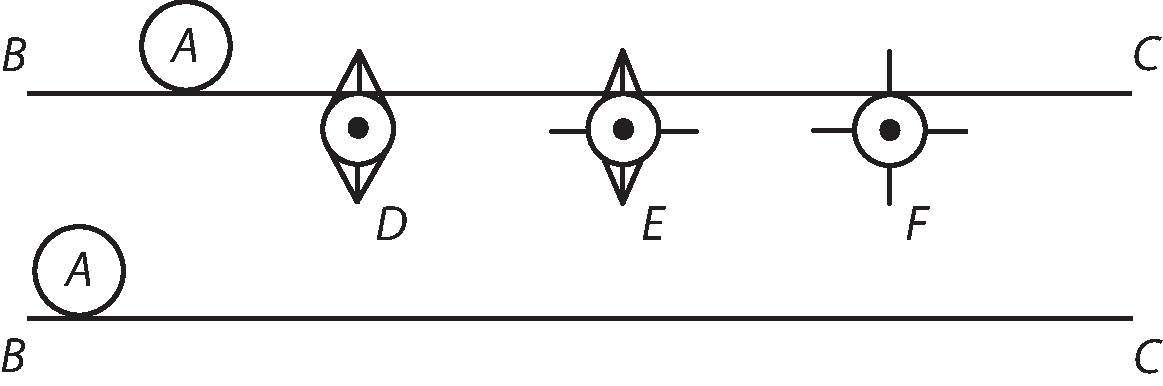
\includegraphics[width=0.63\textwidth]{images/lh0351303_262v-d1.pdf}\\
  \setline{13}  \centering [\textit{Fig. 3}] % \caption{Bildbeschreibung}
    %\end{wrapfigure}
    \pend
    \newpage
\pstart\noindent
c'est \`{a} dire les poids, $\displaystyle p$ et $\displaystyle \pi$ demeurant les \edtext{m\^{e}mes, comme il arrive}{\lemma{m\^{e}mes,}\Bfootnote{\textit{(1)}\ les vi \textit{(2)}\ comme il arrive, \textit{L}}},
quand le m\^{e}me \edtext{corps continue}{\lemma{corps}\Bfootnote{\textit{(1)}\ apr\`{e}s la pr \textit{(2)}\ continue \textit{L}}}
\`{a} passer outre et \`{a} rencontrer des moulinets semblables aux premiers; mais la vitesse estant deminu\'{e}e; les diminutions \edtext{des vitesses}{\lemma{}\Bfootnote{des vitesses \textit{erg.} \textit{L}}}
seront comme les vitesses. Car la premiere vistesse estant \edtext{pos\'{e}e $\displaystyle v$, une autre}{\lemma{pos\'{e}e $\displaystyle v$,}\Bfootnote{\textit{(1)}\ la seconde, \textit{(2)}\ c'est \`{a} dire celle qui \textit{(3)}\  une autre \textit{L}}}
soit appell\'{e}e $\displaystyle (v).$ la diminution de cette 
vistesse sera: \rule[-4mm]{0mm}{10mm}$\displaystyle \frac{\pi}{p+\pi}(v)$
 \rule[-4mm]{0mm}{10mm}\edtext{et $\displaystyle \frac{\pi}{p+\pi}v$ diminution premiere pass\'{e}e sera}{\lemma{et $\displaystyle \frac{\pi}{p+\pi}v$}\Bfootnote{\textit{(1)}\ est diminution pass\'{e}e, \textit{(2)}\ diminution premiere pass\'{e}e  \textit{(a)}\ est  \textit{(b)}\ sera \textit{L}}}
\`{a} \rule[-4mm]{0mm}{10mm}$\displaystyle \frac{\pi}{p+\pi}(v)$ diminution presente, comme $\displaystyle v$ \`{a} $\displaystyle (v)$\edtext{}{\lemma{}\Afootnote{\textit{Am Rand:} (NB)\vspace{-8mm}}} c'est \`{a} dire en raison des vistesses. Cela pos\'{e} je demonstreray aisement que les diminutions des vistesses seront en progression geometrique. Car le \edtext{corps $\displaystyle A$ rencontrant le moulinet $\displaystyle D$ avec la vistesse $\displaystyle v$}{\lemma{corps $\displaystyle A$}\Bfootnote{\textit{(1)}\ rencontre la vistesse \textit{(2)}\ dont le poi \textit{(3)}\ rencontrant [...] vistesse $\displaystyle v$ \textit{L}}}
y perdra la vistesse \rule[-4mm]{0mm}{10mm}\edtext{$\displaystyle \frac{\pi}{p+\pi}v$ et la vistesse}{\lemma{$\displaystyle \frac{\pi}{p+\pi}v$}\Bfootnote{\textit{(1)}\ et rencontrant le moulinet $\displaystyle F$ avec la vistesse $\displaystyle (v)$ \textit{(2)}\ et  \textit{(a)}\ par consequent  \textit{(b)}\ la vistesse \textit{ L}}}%\pend